\documentclass[../thesis.tex]{subfiles}
% Separate preamble for this subfile. This preamble is loaded last, so one can override various functions before \begin{document}

% Better comment extension for Vscode colors these comments differently
% Normal comment color
% * Important information
% ! ALERT
% ? Question
% TODO stuff to do
% // This is strikethrough


\begin{document}
%The topic for this \namecref{sec:aperi_cube} is a new result first put forward by Lagarias, Reeds, and Wang in \cite{lagariasOrthonormalBasesExponentials2000}. However, no proof or reference to the literature was attached. The statement has later been referenced in \cite{liuUniformityNonUniformGabor2003}, although with incorrect reference. After correspondence with one of the original paper's authors, the main result of this \namecref{sec:aperi_cube} has been submitted as a problem for \textsc{The American Mathematical Monthly} \cite{haugeTitle}. It is likely known to the experts that aperiodic tilings by translation of the unit cube exist in all dimensions $d\geq3$; however, the authors of \cite{haugeTitle} are not aware of any solutions in the published literature.  The following will put one solution on the record \cite{haugeTitle}. 

It is likely known to the experts that aperiodic tilings by translation of the unit cube exist in all dimensions $d\geq3$. Lagarias, Reeds, and Wang first put forward the result in \cite{lagariasOrthonormalBasesExponentials2000}. However, no proof or reference to the literature was attached. Later, the same statement appeared in \cite{liuUniformityNonUniformGabor2003}, although with an incorrect reference. Construction of a special kind of tiling in $d=3$ is given in \cite{kolountzakisStudyTranslationalTiling2003}, though with no proof backing up the construction or mention of whether it is an aperiodic tiling. Additionally, the book \cite{zongCubeWindowConvex2006}, which covers cube-tilings, notably lacks any mention of such a tiling as an example. In other words, there is a high possibility that no such constructions exist in the literature. To fill the gap, the following will put one complete solution on the record as a result of joint work with Lagarias \cite{haugeAperiodicTilingTranslations2023} and constitutes the main contribution of the thesis. 

\begin{theorem}[\cite{haugeAperiodicTilingTranslations2023}]
    There exists a translational tiling of unit cubes $I^d + \lambda$ in $\R^d$ for $\lambda\in \Lambda$ in all dimensions $d\geq3$, in which the tiling set $\Lambda$ constitutes an aperiodic tiling.
\end{theorem}

For convenience, we will label unit cubes in the tiling by their corner coordinates which will be given by the vector $x = \brac{x_1,\dots,x_d} \in \R^d$. Note that it is essential that all unit cubes are labeled using the same corner; otherwise, the notation we will employ will lead to overlap. Furthermore, we will use the following notation to describe a unit cube that is parallel to an axis by
\begin{equation*}
    \mathcal{C}\bracMed{x_1,\dots,x_d} = \braqMed{(x_1,\dots,x_d) + (t_1,\dots,t_d) : 0 \leq t_j \leq 1}
\end{equation*} 
where $x\in \R^d$ is the specified corner coordinate. We say that this is an \emph{axis-paralell unit cube}. 

The proof will provide a specific way to construct an aperiodic tiling of unit cubes in any dimension from a fully periodic tiling of unit cubes $\Lambda$ in $\R^d$. We will initially consider a lattice tiling of unit cubes such that all cube-corners will be in an integer lattice, meaning $\Lambda = \Z^d$. The lattice also allows us to employ the notation for an axis-parallel unit cube. Using the following translation, we create the new tiling denoted by $\widetilde{\Lambda}$, which we will show is aperiodic. The translation consists of shifting exactly two specific disjoint columns of unit cubes and leaving the remaining unit cubes in the $\Z^d$-tiling in place. The underlying idea is that the shifted columns create dislocations in the fully periodic tiling of unit cubes $\Lambda$. We can think of these dislocations as line or skew-line defects. The critical observation is that the position of the defects can be detected locally and that these positions move when $\widetilde{\Lambda}$ undergoes a translation. Since translated tilings of $\widetilde{\Lambda}$ will differ from the original tiling $\widetilde{\Lambda}$, we have that $\widetilde{\Lambda}$ will have no non-trivial translation symmetry, and hence must necessarily be aperiodic. 

\begin{remark}
    The use of \emph{column} in this \namecref{sec:aperi_cube} differs from how the term has been used in the rest of the thesis. Here, a column is considered to be a one-dimensional column of unit cubes in one of the $d$ coordinate directions. As an example, for $d=2$, what we previously denoted as a row or a column of unit cubes is now considered a column of unit cubes in either the first or second coordinate direction, respectively.
\end{remark}

\begin{proof}
Before generalizing it to higher dimensions, we prove the result for dimension $d=3$. Here we displace two columns of unit cubes with corner coordinates 
\begin{align*}
    \bracMed{m_1,0,1},& \quad m_1 \in \Z,\\
    \bracMed{0,1,m_3},& \quad m_3 \in \Z,
\end{align*}
shifting each of them with the respective translation vectors $\upsilon' = \brac{\frac{1}{2},0,0}$ and $\upsilon'' = \brac{0,0,\frac{1}{2}}$ so that
\begin{align*}
    \bracMed{m_1,0,1} \xlongrightarrow[]{\upsilon'} \bracMed{m_1 + \frac{1}{2} ,0,1}, \quad  &\text{ for all } m_1 \in \Z,\\
    \bracMed{0,1,m_3} \xlongrightarrow[]{\upsilon''} \bracMed{0,1,m_3 + \frac{1}{2} },    \quad  &\text{ for all }  m_3 \in \Z.
\end{align*}
Observe that the column of unit cubes covers exactly the same set after the translation since the translation is in the same direction as the column itself
\begin{align*}
    \braqMed{ \bracMed{x_1, 0+t_2,1+t_3} : 0 \leq t_j \leq 1, x_1\in\R} \xlongrightarrow[]{\upsilon'} & \braqMed{ \bracMed{x_1, 0+t_2,1+t_3} : 0 \leq t_j \leq 1, x_1\in\R},\\
    \braqMed{ \bracMed{0+t_1,1+t_2,x_3} : 0 \leq t_j \leq 1, x_3\in\R} \xlongrightarrow[]{\upsilon''} & \braqMed{ \bracMed{0+t_1,1+t_2,x_3} : 0 \leq t_j \leq 1, x_3\in\R}.
\end{align*}
In addition, note that both shifted columns are disjoint in $\R^3$ since their middle corner coordinates $x_2$ differ by a non-zero integer. Hence, the new tiling $\widetilde{\Lambda}$ is still a cube-tiling of $\R^3$. To show that $\widetilde{\Lambda}$ is an aperiodic tiling, consider the following. Let $\tau=\brac{\tau_1,\tau_2,\tau_3}\in \R^3$ be a vector which we associate with the translation
\begin{equation*}
    \mathbf{T}_\tau \bracMed{x} = x+\tau = \bracMed{x_1+\tau_1, x_2+\tau_2, x_3+\tau_3},
\end{equation*}
where $x\in \R^3$ is the point on which the translation acts. If the $\mathbf{T}_\tau \brac{x}$ maps cube-corners to cube-corners, then the tiling will be invariant under the translation. From this, we will show that $\tau=\brac{0,0,0}$ is the only vector that preserves the set of cube-corners making $\widetilde{\Lambda}$ an aperiodic tiling of unit cubes. 

%OLD: We first show that the translation vector $\tau \in \Z^3$. Consider a $2\times 2\times 2$ block of $8$ unit cubes in $\widetilde{\Lambda}$, which do not intersect any part of our translated columns. Note that all unit cubes in our block have integer coordinates. When translating the block, its image under the translation must also be a $2\times 2\times 2$ block of $8$ unit cubes in $\widetilde{\Lambda}$. Since our shifted columns are disjoint, there will be at most $4$ unit cubes from our shifted columns, while the remaining unit cubes must still have integer coordinates. As such, $\tau$ maps an integer vector to another integer vector. That is, $\tau$ maps some cube-corner from the initial block to a cube-corner in the image block, which has an integer corner vector. Hence, $\tau \in \Z^3$. 
We first show that the translation vector $\tau \in \Z^3$. Consider a $2\times 2\times 2$ block of $8$ unit cubes in $\widetilde{\Lambda}$, which do not intersect any part of our translated columns. Note that all unit cubes in our block have integer coordinates. When translating the block, its image must also be a $2\times 2\times 2$ block of $8$ unit cubes in the image of $\widetilde{\Lambda}$ under the translation. Now, comparing the original $\widetilde{\Lambda}$ with the image of $\widetilde{\Lambda}$ under the translation shows the following. Since our shifted columns are disjoint, there might be at most $4$ unit cubes from the image of the block in the shifted columns of the original $\widetilde{\Lambda}$. However, more importantly, the remaining unit cubes must still have integer coordinates. As such, $\tau$ maps an integer vector to another integer vector. That is, $\tau$ maps some cube-corner from the initial block to a cube-corner in the image block, which has an integer corner vector. Hence, $\tau \in \Z^3$. 

Secondly and last, we show that the translation vector $\tau = \brac{0,0,0}$. We first claim that $\tau$ must map each of the two shifted columns into itself. Before proving the claim, we show how the result follows. Therefore, assume the claim is valid. Observe that the translation which maps the first shifted column of unit cubes to itself is one with a translation in the same direction as the shift. That is, we must have $\tau' = (\tau'_1,0,0)$ for any $\tau'_1\in \Z$ since
\begin{equation*}
    \bracMed{m_1 + \frac{1}{2} ,0,1} \xlongrightarrow[]{\tau'} \bracMed{m_1+\tau'_1 + \frac{1}{2} ,0,1}, \quad \text{ for all } m_1 \in \Z,\\
\end{equation*}
which is still the same column of unit cubes as $m_1+\tau'_1\in\Z$. Similarly, for the second shifted column, we must have $\tau'' = (0,0,\tau''_3)$ for any $\tau''_3\in \Z$ since 
\begin{equation*}
    \bracMed{0,1,m_3 + \frac{1}{2} } \xlongrightarrow[]{\tau''} \bracMed{0,1,m_3+\tau''_3 + \frac{1}{2} } , \quad \text{ for all } m_3 \in \Z,\\
\end{equation*}
which is still the same column of unit cubes as $m_3+\tau''_3\in\Z$. To satisfy both translations described by $\tau'$ and $\tau''$ at the same time we must have, $\tau_1 = 0$ from $\tau''$, and $\tau_3 = 0$ from $\tau'$. Last, since $\tau_2'=\tau_2'' = 0$ we have $\tau_2=0$. Hence $\tau = \brac{0,0,0}$.

To show the claim, note that since $\tau\in\Z$, it will, for each cube-corner vector, preserve both; the shifted part, or in this case, the fractional part of a coordinate and also its position in the cube-corner vector. As it is only the two shifted columns that have non-zero fractional parts in the tiling $\widetilde{\Lambda}$, we have that the fractional part will always be in the first coordinate position for the first column, and always the third coordinate position for the second column. Using that $\tau\in\Z$ means that if our initial tiling vector $\tilde{\lambda} \in \widetilde{\Lambda}$ has a non-zero fractional part in some coordinate position, then the image vector of $\tilde{\lambda}$ will have an equal non-zero fractional part in the same coordinate position. The converse is also true. 

To show the $n$-dimensional case, we modify the above arguments. Take the two columns of unit cubes in the initial $\Z^d$-tiling to be the ones with corner coordinates
\begin{align*}
    \bracMed{m_1,1,0, \dots,0}, & \quad m_1 \in \Z,\\
    \bracMed{0,\dots,0,1,m_d},& \quad m_d \in \Z,
\end{align*}
and using a similar shift of $\upsilon' = \brac{\frac{1}{2},0,\dots,0}$ and $\upsilon'' = \brac{0,\dots,0,\frac{1}{2}}$ to get
\begin{align*}
    \bracMed{m_1,1,0, \dots,0} \xlongrightarrow[]{\upsilon'} \bracMed{m_1+\frac{1}{2}, 1, 0, \dots, 0}, \quad  &\text{ for all } m_1 \in \Z,\\
    \bracMed{0,\dots,0,1,m_d} \xlongrightarrow[]{\upsilon''} \bracMed{0, \dots, 0, 1, m_d+\frac{1}{2}},    \quad  &\text{ for all }  m_3 \in \Z.
\end{align*}
Then, using the exact same arguments, but now with a $\overbrace{2\times \dots \times 2}^{d-\text{times}}$ block of unit cubes, and that the only column preserving translations $\tau'$ and $\tau''$ must be
\begin{align*}
    \tau' =& \bracMed{\tau'_1,0,\dots,0 }, \quad \tau'_1 \in \Z,\\
    \tau'' =& \bracMed{0,\dots,0,\tau''_d}, \quad \tau''_d \in \Z,
\end{align*}
shows that the translation vector $\tau=\brac{0,\dots,0}$ is the zero-vector.
\end{proof}

\begin{figure*}[h!]
    \centering
    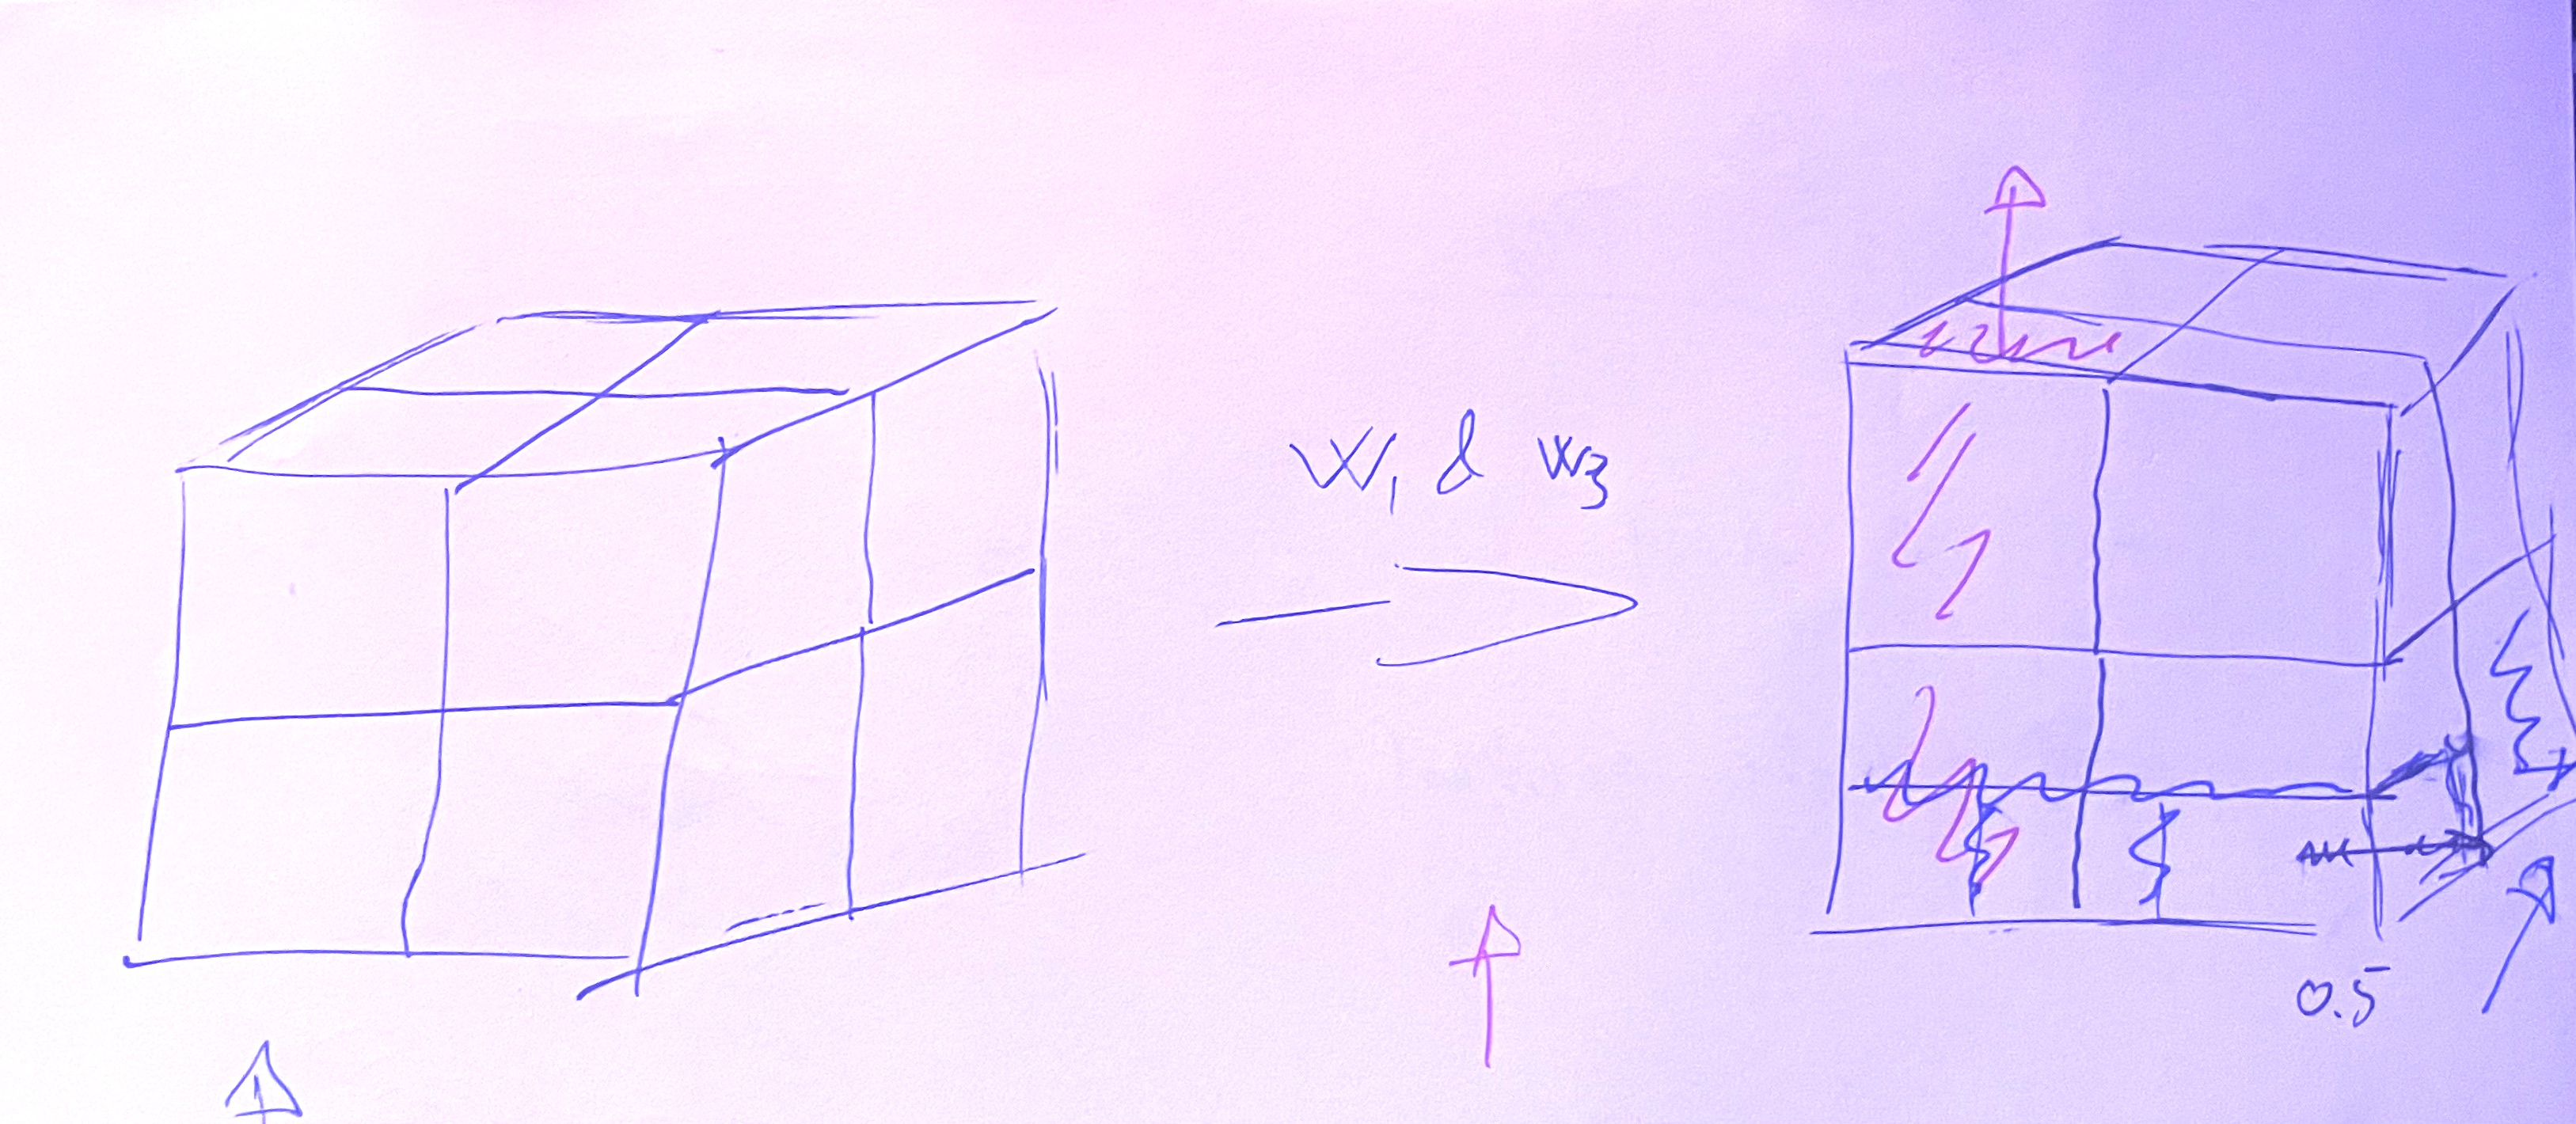
\includegraphics[width=0.87\linewidth]{aper_yeye.jpg}
    \caption{TEXTTEXT lorum blabla, figure placement somewhere nice}
    \label{fig:aperi_cube}
\end{figure*}

Illustrated in FIG:A is the initial lattice tiling $\Lambda$, and illustrated in FIG:B is the constructed aperiodic tiling $\widetilde{\Lambda}$ after translation of $\upsilon'$ and $\upsilon''$. The latter figure also shows that there can be no more than four unit cubes from the shifted columns in a $2\times 2\times 2$ block of cubes. 

\end{document}